\chapter{System Design}

\section{Introduction}
This chapter details the design of a Doppler wind LiDAR system. As discussed in the introduction and scope of this report, the system is a benchtop prototype whose purpose is to make the sensitivity of a DWL measurable and attributable to specific component and architecture choices. As such, the primary considerations will be noise-levels, sensitivity, and the overarching principles of physics governing DWL systems. This system design will thus not include the design of housing for field deployment, nor will it be concerned with real-time post-processing pipelines for the system's data (which would be required in a field-deployed system). Furthermore, several key components that would be typical in a scientific- or industry-grade, field-deployable DWL system are deliberately omitted in order to reduce costs, at little functional expense for a benchtop system. Where possible, the system was made extensible for future iterations and field deployment.

First \autoref{sec:design-sysArch} gives an overview of the architecture chosen, as synthesised from the various architecture types reviewed in \autoref{sec:litReview}, and with respect to the project's overarching goals. Thereafter, \autoref{sec:design-sysReqs} discusses the functional and performance requirements of the system. Finally, section \ref{sec:design-ComponentChoices} details the specific components chosen to meet these requirements. 

\section{System Architecture}
\label{sec:design-sysArch}
From the reviewed literature in \autoref{sec:litReview}, it was decided that an \textbf{all-fibre, coherent detection, continuous-wave, monostatic} DWL system with \textbf{balanced detection} would be built, with sampling and digitisation to be handled by a benchtop oscilloscope, and post-processing done on a laptop computer. This section details why these architectural choices were made, using summarised information from \autoref{sec:litReview} with respect to the project goals, and discusses any significant implications for the system. 

\subsection{Coherent detection}
\label{sec:design-sysArch}
The direct detection technique requires the
Rayleigh/Mie scattering ratio and temperature, an absolutely stabilised laser, etalon
control to 1 milli-Kelvin, and very precise physical alignment and calibration
\cite{korb_theory_1998,colberg_diode-laser-based_2026,werner_doppler_2005}. These present substantial challenges to an undergraduate project, particularly the stabilised laser and etalon temperature control. The one advantage which direct detection holds, which is the capability of using molecular backscatter when aerosol backscatter is not available, is irrelevant in an aerosol-rich controlled lab environment, which is the only environment this system will be tested in.

By contrast, coherent detection is far more common in the literature, and thus has more practical information and sources for components. Furthermore, mixing with the LO also permits shot-noise-limited operation through the effective amplification of the return signal, and rejects unwanted light not
mode-matched to the LO \cite{hill_remote_nodate} (e.g. other LiDAR systems, or the sun), thus reducing sources of potential interference. The architecture thus lends itself to a more elegant, direct method of measuring the Doppler shift, via optical mixing and subsequent detection. 

For these reasons, a coherent detection system was chosen for this project build. 

\subsection{Homodyne mixing}
Homodyne mixing places the Doppler shift at baseband with no additional frequency shift, and no additional components necessary, whereas heterodyne operation requires an acousto-optic
modulator (AOM) in the LO or transmit arm
\cite{harris_role_1998,abdelazim_development_2015}. The tradeoff  is the sign ambiguity as discussed in \autoref{sec:lit-homohetero}, where only the velocity \textbf{magnitude} is
measured in a homodyne system, whereas a heterodyne system can resolve the direction.

For a benchtop-scale system which primarily aims to present the working principles of a DWL system and a sensitivity analysis, and where the direction of the flow being measured will always be known, it is not necessary to recover signed velocity. Adding an AOM thus adds needless complexity, and adds an additional unnecessary cost to a budget-constrained project. Crucially however, the addition of an AOM for a future iteration of the system is simple, and does not require the redesign of any parts of the current system. For these reasons it was thus decided to omit the AOM, and to therefore construct a \textbf{homodyne} coherent detection system.

\subsection{Balanced detection}
As discussed in \autoref{sec:lit-BalancedDetection}, balanced detection holds the advantage of providing a 3dB improvement in SNR (in shot-noise limited operation) as compared to single ended detection. It also allows RIN to be largely cancelled, further allowing SNR improvement, and allowing the system to better approach the shot-noise limit (see Appendix \ref{appendix:RIN}). For these reasons, it was decided that a balanced detection setup would be used.

\subsection{Monostatic optics}
For this project, it was decided to use a monostatic optical configuration - where a single aperture serves both transmit and receive, separated by a fibre
circulator, with no second lens and no alignment of two lenses necessary. A bistatic arrangement would
keep transmit-optics back-reflections away from the detector, at the cost of greatly increased alignment complexity
\cite{cariou2006laser,harris_role_1998,bennett_doppler_2003}, as well as the additional cost of 2 sets of optics, and equipment needed for alignment. The accepted
tradeoff here is thus that back-reflections from the transmit path reach the detector and
raise the noise floor through PIIN (see \autoref{sec:lit-linewidth}).

\subsection{Continuous-wave operation}
Pulsed systems are ineffective below tens of metres because the pulse length is typically at least as long as this range \cite{hill_remote_nodate}. a CW system needs no pulse or receive timing, which simplifies design and can reduce costs (due to lower component count). It is also the more effective of the two at short range. One of the significant performance costs of a CW system however is reduced spatial resolution, particularly at long ranges, as spatial resolution is defined by focus rather than gating with timing (see \autoref{sec:lit-pulsedCW}). Seeing as a benchtop system requires operation at short ranges in the order of tens of centimeters to one or two meters, a CW system will be best suited here due to its simplicity, and its advantages at short range, as well as the irrelevance of long-range limitations.

\subsection{All-fibre construction}
For this project it was decided that an all-fibre construction would be used - meaning that fibre optic cables would be used to transmit the LO and emission beams, and return signals, rather than transmitting the beams through free-space. Single-mode fibre makes the mode-matching between LO and return that coherent detection requires automatic, removes free-space alignment complexities, and gives access
to widely and cheaply available telecom components
\cite{bennett_doppler_2003,abari_all-fiber_2014,abdelazim_development_2015}. Non polarisation-maintaining fibre is used, owing to cost considerations as compared to polarisation-maintaining fibre.
The accepted tradeoff of standard (non-polarisation-maintaining) fibre is that the polarisation of LO and return is not fixed, which will reduce the heterodyne efficiency of the system, and thus reduce the measureable Doppler peak \cite{cariou2006laser}. 


\subsection{System Architecture Diagram}
\autoref{fig:design-architecture} below shows a functional block-diagram of the system's decided-upon architecture. In this diagram, the signal path can clearly be seen from laser source, through the splitter (splitting into LO and transmit beam). Thereafter the transmit beam gets routed via port 1 --\textgreater 2 of the circulator to the monostatic optics, which also receives the backscatter signal to be routed via port 2 --\textgreater 3 of the circulator. The local oscillator and backscatter signals are mixed in the optical mixer, and then detected by a balanced photodetector, from which the final output beat signal can be sampled and processed. 
\begin{figure}[H]
\centering
\resizebox{\textwidth}{!}{%
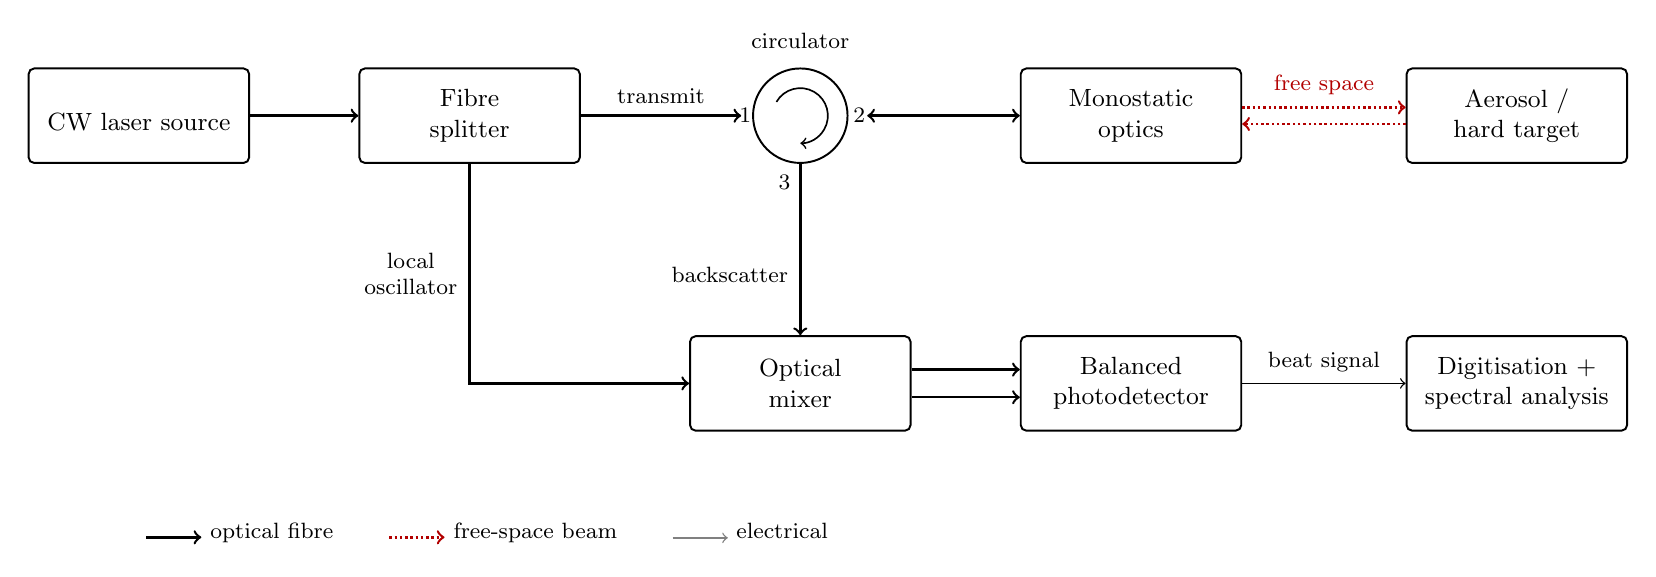
\begin{tikzpicture}[
  font=\small, line width=0.7pt,
  block/.style={draw, rounded corners=2pt, align=center, minimum height=1.2cm,
                minimum width=2.8cm, inner sep=5pt},
  fibre/.style={->, line width=0.9pt},
  fibreBoth/.style={<->, line width=0.9pt},
  free/.style={->, line width=0.9pt, red!70!black, densely dotted},
  elec/.style={->, line width=0.5pt, gray},
  leak/.style={->, line width=0.7pt, red!70!black, dashed},
  lbl/.style={font=\footnotesize, align=center, inner sep=2pt}
]

% ---- top row ----
\node[block] (laser) at (0,0)  {\\CW laser source};
\node[block] (cpl)   at (4.2,0) {Fibre\\splitter};
\node[draw, circle, minimum size=1.2cm] (circ) at (8.4,0) {};
\draw[->, line width=0.6pt] (8.4,0) ++(150:0.35) arc (150:-90:0.35);
\node[lbl] at (7.7,0)    {1};
\node[lbl] at (9.15,0)    {2};
\node[lbl] at (8.2,-0.85) {3};
\node[lbl] at (8.4,0.95)  {circulator};
\node[block] (coll)  at (12.6,0) {Monostatic\\optics};
\node[block] (tgt)   at (17.5,0) {Aerosol /\\hard target};

\draw[fibre] (laser.east) -- (cpl.west);
\draw[fibre] (cpl.east)   -- (7.65, 0) node[midway, above=2pt, lbl] {transmit};
\draw[fibreBoth] (9.25, 0)  -- (coll.west);
\draw[free] ([yshift= 3pt]coll.east) -- ([yshift= 3pt]tgt.west)
  node[midway, above=2pt, lbl] {free space};
\draw[free] ([yshift=-3pt]tgt.west)  -- ([yshift=-3pt]coll.east);

% ---- bottom row ----
\node[block] (comb) at (8.4,-3.4)  {Optical\\mixer};
\node[block] (det)  at (12.6,-3.4) {Balanced\\photodetector};
\node[block] (dsp)  at (17.5,-3.4) {Digitisation +\\spectral analysis};

\draw[fibre] (cpl.south) |- (comb.west)
  node[pos=0.25, left=2pt, lbl] {local\\oscillator};
\draw[fibre] (circ.south) -- (comb.north)
  node[pos=0.65, left=2pt, lbl] {backscatter};
\draw[fibre] ([yshift= 5pt]comb.east) -- ([yshift= 5pt]det.west);
\draw[fibre] ([yshift=-5pt]comb.east) -- ([yshift=-5pt]det.west);
\draw[elec, black] (det.east) -- (dsp.west) node[midway, above=2pt, lbl] {beat signal};

% ---- legend ----
\node[lbl, anchor=west] at (0,-5.3) {%
  \tikz\draw[->, line width=0.9pt] (0,0)--(0.7,0); optical fibre \qquad
  
  \tikz\draw[->, line width=0.9pt, red!70!black, densely dotted] (0,0)--(0.7,0); free-space beam \qquad
  
  \tikz\draw[->, line width=0.5pt, gray] (0,0)--(0.7,0); electrical};
\end{tikzpicture}}
\caption{Block diagram of the chosen architecture: all-fibre, coherent,
continuous-wave, monostatic, homodyne, with balanced detection}
\label{fig:design-architecture}
\end{figure}

\section{System Requirements Analysis}
\label{sec:design-sysReqs}
Now that a system architecture has been decided on, requirements which are specific to this choice of architecture, and which are related to the project goals can be synthesised. The requirements for the system are divided into two sets: functional requirements, which define the ideal outcomes which are desired from the system, and performance requirements, which define specific metrics which are to be measured and quantified with respect to the goals of the functional requirements. 

\subsection{Functional requirements}
\begin{enumerate}

  \item Measure the line-of-sight velocity of a target from the          Doppler shift of coherently detected backscatter,
        using a monostatic all-fibre homodyne architecture with balanced detection and continuous-wave operation.
  \item Operate on both a diffuse hard target of known velocity and on air seeded with smoke or fog. 
  \item Produce a velocity estimate from a recorded spectrum using a stated, reproducible detection criterion (threshold relative to the system's noise floor).
\end{enumerate}

\subsection{Performance requirements}
From the desired functional requirements, a set of performance requirements can be synthesised; these are given in \autoref{tab:requirements} below along with the IDs of the tests which will verify them. 

%It must be noted again here that this project's goals chiefly concern the measurement and characterisation of noise and SNR in a constrained DWL system build, and how these aspects relate to component choice. As such, the majority of these requirements are concerned with the characterisation of the system relative to an ideal system, and thus the quantification of the system's limitations - rather than attempting to achieve performance specifications which will allow all the functional requirements to be met. 
\begin{table}[H]
\centering
\small
\begin{tabular}{|p{0.5cm}|p{3cm}|p{9cm}|p{1.7cm}|}
\hline
\textbf{ID} & \textbf{Requirement} & \textbf{Value} & \textbf{Verified by} \\ \hline
P2 & Detector noise & approaching ideal shot-noise-limited behaviour: total
     detector noise (electronic noise + residual RIN after balanced
     detection) within \SI{1}{\decibel} of the shot-noise limit
    & A1, A2 \\ \hline
 P4 & Phase-induced intensity noise (PIIN) & Level (in dB) and spectral shape measured;
 agreement with the path-mismatch model of \cite{harris_role_1998}
    within \SI{6}{\decibel} & B \\ \hline
P3 & Total system noise & Total noise floor (shot + electronic + residual RIN + PIIN) quantified with respect to the shot-noise limit, and sources of excess noise described and characterised & B \\ \hline
 P1 & Velocity detection on a hard target & Doppler peak detected at $ \gg 5\times\sigma$ (5 times the noise standard deviation) above the  mean, at $N \leq 1000$ averages, for a hard target 10cm away from laser emission & C \\ \hline
P5 & Low-velocity limit & Minimum resolvable LOS speed of $\leq$ \SI{0.1}{\metre\per\second} on a hard target & C \\ \hline
P6 & Detection of wind-speed in seeded air (smoke or fog) & Doppler peak detected at $ \gg 5\times\sigma$ (5 times the noise standard deviation) above the  mean, at $N \leq 10 000$ averages 
& D \\ \hline
P7 & Velocity accuracy & Doppler velocity within 5\% of ground-truth velocity of target (hard target and seeded flow) & C, D \\
\hline
\end{tabular}
\caption{Performance requirements and their verification tests.}
\label{tab:requirements}
\end{table}

\section{Component Choices}
\label{sec:design-ComponentChoices}
This section details the specific component selections which were made for the system. These selections were made to best suit the functional and performance requirements of the system. It must be noted that this project is constrained when compared to typical scientific or industrial DWL systems. As such, many component choices were driven by cost, availability, and time-frame considerations, rather than simply their suitability for the system. This is however a suitable approach for the goals of the project, which are to illustrate the principles and physics involved in a DWL system, and to quantify system performance with respect to component choices. 
\subsection{Laser Source}
    The selection of an appropriate laser source is critical to ensure good performance of a DWL system. There are numerous properties of a laser source which should be considered, and which will be detailed in this section. After discussion on these properties, a suitable laser source is selected. 

    \subsubsection{Wavelength}
    There are many suitable wavelengths for DWL systems, as detailed by Cariou et. al \cite{cariou2006laser}. There is much discussion around SNR optimisation and backscatter maximisation for varying wavelengths \cite{bennett_doppler_2003}, however owing largely to practical advantages, a wavelength of 1550nm has emerged as a common choice for both commercial and scientific DWL systems \cite{abari_all-fiber_2014}. Fiber optics telecommunications  commonly operate at this wavelength - thus making components designed for this wavelength readily commercially available and significantly cheaper than alternatives \cite{cariou2006laser}, \cite{abdelazim_development_2015}, \cite{hill_remote_nodate}. Additionally, laser beams at 1550nm are eye-safe at significantly higher power levels (up to multiple Watts), compared to shorter wavelengths \cite{cariou2006laser}, reducing safety concerns. For this reason it was decided that a 1550nm laser source would be used for this project. 
    
    \subsubsection{Power Level}
    % EDFAs
    % Backscatter intensity 
    As previously discussed, the ability of a DWL system to measure wind-speed depends on the measurement of aerosol backscatter of the emitted beam. 
    
    The time-averaged power of the backscatter signal into a receiver can be expressed as \cite{hill_remote_nodate}:
    
        \begin{equation}
            P_s = \pi P_t \beta(\pi) \lambda
            \label{eqn:backscatterPower}
        \end{equation}

    Where $P_s$ is the time averaged backscatter signal power, $\beta(\pi)$ is the atmospheric scattering coefficient (evaluated at $\pi$, i.e. scattering at $\pi$ radians, back towards the source), and $\lambda$ is the wavelength of the transmitted light. Note that $\beta(\pi)$ also holds a wavelength dependence, and thus $P_s$ does not necessarily scale linearly with increasing wavelength, as the equation may suggest, but instead resolves to a near cancellation of the wavelength dependence between some frequency ranges \cite{bennett_doppler_2003}.
    
    It can be seen in \autoref{eqn:backscatterPower} that there is a linear dependence on $P_t$, the power of the transmitted beam. Thus, a higher-powered transmit laser source would give a larger return signal to be measured, increasing the sensitivity of the system by increasing the SNR of the system \cite{bennett_doppler_2003}. 

    A setup commonly used to achieve higher emitted laser power here is the master-oscillator power-amplifier (MOPA) configuration \cite{cariou2006laser}, \cite{bennett_doppler_2003}. This separates the functions of the laser source - allowing for a low-power, highly coherent, narrow linewidth laser source to be used as a master-oscillator and an amplifier to increase the power levels of the master oscillator beam, while maintaining its spectral purity. This also allows the local oscillator to be derived from the master oscillator, eliminating the need to have two separate laser sources - one for LO, one for output - which would need to have a stable frequency relationship \cite{cariou2006laser}, something which requires careful design to achieve, as illustrated by Colberg et al. \cite{colberg_diode-laser-based_2026}.  

    As noted by Bennett, such power amplifiers (commonly Erbium-doped fiber amplifiers; EDFAs) make up a significant portion of the cost of a DWL system. Indeed, more than 20 years after the writing of Bennett's paper, the cost of EDFAs remain prohibitively expensive for a project at this scale. For EDFA systems which are able to amplify signals to hundreds of milli-Watts or multiple Watts (which is a typical power level for such a system \cite{abdelazim_development_2015}\cite{cariou_leosphere_nodate}\cite{cariou2006laser}), current prices range in the thousands to tens of thousands of USD (see Appendix). 
    
     For this reason, the use of a power amplifier for the laser source is disqualified for this project on the grounds of cost. The system was however designed such that the addition of such an amplifier would be possible at a later stage.
     
     Due to the relatively low powers available for laser sources without power amplification (in the tens of milli-Watts), other avenues to improve detection sensitivity will be required. Bennett identifies another option for increasing the sensitivity of a DWL system - which is to average over many returns \cite{bennett_doppler_2003}. This is the approach which will be taken for this project. Additionally, owing to this constraint in laser source power, all tests which concern wind-speed measurement in air will be performed using air seeded with smoke and/or fog. This will increase backscatter levels by increasing $\beta(\pi)$ in \autoref{eqn:backscatterPower}, and thus reduces the need for the power amplifier for this benchtop-scale system. The level of seeding required for a lower-power laser source to detect wind-speed is one of the investigations of this project.

    \subsubsection{Linewidth}
    \label{sec:lit-linewidth}
    Linewidth can be seen as a measure of the spectral purity of a laser source, and is one of the most critical parameters in the design of a DWL system. A narrow linewidth is highly desirable for DWL applications, as this will significantly reduce the phase-induced intensity noise (PIIN) in a DWL system, and allow the system to therefore have a better SNR and sensitivity to detect small backscatter signals. Furthermore, the linewidth of a laser source has a significant effect on how broad the returned backscatter signal's Doppler shifted peak is, particularly at longer ranges. This will result in the system having worse precision, and not being able to resolve turbulence in the air as well. For a full discussion on the mathematical and physical meaning of linewidth, as well as a treatment on how linewidth affects PIIN and the broadened peak, see Appendix \ref{appendix:PIIN}. Cariou et al. make the claim that linewidths typical of DFB diodes (0.5 - 5MHz, see \autoref{tab:design-laser-sources}) disqualify them for use in CW DWL systems due to their PIIN, however, Bennett shows that indeed a DFB source with a linewidth of 1.4MHz can be used for these purposes, provided careful attention is given to other design considerations, such as optical fiber path length matching \cite{bennett_doppler_2003}. The analysis of noise in the system, and the associated constraints arising from the use of a comparatively wider linewidth laser source indeed forms a key part of this project, owing to budget considerations, as will be discussed below and in \autoref{sec:noiseAnalysis}.
    
    

    \subsubsection{Laser source types and selection}
    There are many types of laser sources available on the market. In the selection of a laser source for this project, the primary driver was cost and availability, with the design goals being to maximise power level and minimise linewidth, while fixing the wavelength at 1550nm. After selecting the best available laser source for these parameters, the performance of the laser source will then be analysed, and recommendations based on its properties and performance can then be made. 

\begin{table}[H]
\centering\small
\renewcommand{\arraystretch}{1.2}
\begin{tabular}{@{}|p{2.6cm}|p{1.9cm}|p{1.7cm}|p{6.0cm}|p{2.2cm}|@{}}
\hline
\textbf{Source type} & \textbf{Linewidth (typ.)} & \textbf{Power, unamplified} & \textbf{Noise and practical notes} & \textbf{Indicative cost (USD)} \\
\hline
Fabry--P\'erot laser diode &
multi-mode; not single-frequency &
\SIrange{10}{100}{\milli\watt} &
Multi-mode, Unsuitable for coherent detection due to this. \cite{harris_role_1998}.  &
$<100$ \\
\hline
DFB laser diode &
\SIrange{0.5}{5}{\mega\hertz} &
\SIrange{10}{40}{\milli\watt} &
Relaxation peak \SI{\sim1}{\giga\hertz}, far above the Doppler band, thus is RIN flat and low in the frequency band of interest \cite{cariou2006laser}. Needs external driver and temperature controller. &
\numrange{100}{1000} (module) \\
\hline
Planar external-cavity semiconductor &
$<1$ to \SI{15}{\kilo\hertz} &
\SIrange{10}{30}{\milli\watt} &
Integrated driver, marketed for wind lidar.&
quote only; low thousands \\
\hline
Er-doped DFB fibre laser &
$<0.1$ to \SI{10}{\kilo\hertz} \cite{harris_role_1998} &
\SIrange{10}{40}{\milli\watt} &
Common source of choice for CW anemometry due to narrow linewidth \cite{cariou2006laser,hill_remote_nodate, abdelazim_development_2015}. Relaxation peak near \SI{1}{\mega\hertz}, so higher RIN in the frequency band of interest \cite{cariou2006laser}. &
quote only; tens of thousands \\
\hline
\end{tabular}
\caption{Laser source classes at \SI{1550}{\nano\metre}. Linewidths and powers are typical of commercial devices; approximate costs are as of September 2026 and exclude drivers, controllers and import costs.}
\label{tab:design-laser-sources}
\end{table}

From these available laser source options, it was decided that a DFB laser diode would be used. While the wider linewidth, as compared to Planar external-cavity semiconductor diodes or Er-doped DFB fibre lasers is likely to substantially increase PIIN, measures such as fiber length matching will be investigated to reduce PIIN for lower-range, tabletop operation (see \autoref{sec:testingPIIN}), and these narrow linewidth sources are out of budget for this project. 

The final specifications of the obtained laser diode are as follows:
\begin{table}[H]
	\centering
	\label{tab:dfb-laser}
	\begin{tabular}{@{}ll@{}}
		\toprule
		\textbf{Parameter} & \textbf{Value} \\
		\midrule
		Wavelength                  & 1550~nm \\
		Rated output power          & 20~mW \\
		Linewidth                   & 2~MHz \\
		Operating current at 20mW & 58~mA \\
		Fibre output                & Single-mode, FC/APC \\
		\bottomrule
	\end{tabular}
	\caption{Key properties of the selected DFB laser diode
		(BFLD-1550-20SM-FA2). Full specifications are given in
		\autoref{appendix:laser}.}
\end{table}

\subsection{Laser driver and temperature control}
In order to keep the laser diode at a constant operating point, a constant current source must be used to drive it, and a temperature controller should be used. Temperature and current fluctuations present in the laser output as fluctuations in wavelength and output power \cite{Gwinner2024}, which can have a significant effect on the noise in measurements, particularly in a sensing system, such as a DWL, for which measurements of very small signals is required.

 Perhaps the greater consideration however is the safety of the laser diode. The laser diode chosen forms the single biggest expense in this DWL system, and thus protecting it is of vital importance to this project. Laser diodes are extremely sensitive to transients and overvoltage events, which can easily damage them \cite{Gwinner2024}. Circuitry for these ends may be custom-designed and manufactured as a PCB, however, this is a complex process, and is best-suited to systems where commercially available driver and temperature control circuitry is unsuitable. Thus, for this project it was decided that off-the-shelf circuitry would be used for these ends, so that the expensive laser diode is safeguarded against possible custom design flaws or oversights of a first-time designer. Commercial off-the-shelf units integrate soft-start circuitry, current control, current monitoring, protection against overvoltage and overcurrent events and transients into a single package.
 
 The Koheron DRV200S-A-200 laser driver was chosen, due to its very low noise characteristics, and the suitability of the current range and limit for the BFLD-1550-20SM-FA2 laser diode chosen above. The Koheron TEC100L-50 temperature controller was chosen from the same supplier, and has an adequate setpoint range and stability for the project. The respective specifications of the selected laser driver and  temperature controller are given below:
 
 \begin{table}[H]
 	\centering
 	\begin{minipage}[t]{0.48\textwidth}
 		\centering
 		\label{tab:drv200s}
 		\begin{tabular}{@{}ll@{}}
 			\toprule
 			\textbf{Parameter} & \textbf{Value} \\
 			\midrule
 			Current range             & 0--200~mA \\
 			Current limit (adj.)      & 65--300~mA \\
 			Noise density (1~kHz)     & 270~pA/$\sqrt{\text{Hz}}$ \\
 			RMS noise (10~Hz--1~MHz)  & 265~nA \\
 			Temperature coefficient   & 30~ppm/$^\circ$C \\
 			\bottomrule
 		\end{tabular}
 		\caption{Key specifications of the Koheron DRV200S-A-200
 			laser diode driver.}
 	\end{minipage}
 	\hfill
 	\begin{minipage}[t]{0.48\textwidth}
 		\centering
 		\label{tab:tec100l}
 		\begin{tabular}{@{}ll@{}}
 			\toprule
 			\textbf{Parameter} & \textbf{Value} \\
 			\midrule
 			TEC current               & $\pm$1.15~A \\
 			Setpoint range            & 10--40~$^\circ$C \\
 			24~h stability            & 0.005~$^\circ$C \\
 			Temperature coefficient   & 0.002~$^\circ$C/$^\circ$C \\
 			Supply voltage            & 5~V \\
 			\bottomrule
 		\end{tabular}
 		\caption{Key specifications of the Koheron TEC100L-50
 			temperature controller.}
 	\end{minipage}
 \end{table}
 
 \subsection{Detector}
 Balanced detectors typically include two matched photodiodes, connected differentially to a low-noise transimpedance amplifier which converts the photodiode current into a measurable voltage. Seeing as the beat signal which will be measured is in the order of mega-Hertz in frequency, much care needs to be taken when designing the electronic circuitry of the detector to avoid parasitic effects, such as stray capacitance and inductance, which can cause amplifier instability and limit bandwidth, as well as susceptibility to electromagnetic interference. Given the difficulty of proper RF design, to simultaneously achieve high bandwidth, low noise and high common-mode rejection in a custom design, a commercial balanced detector was selected so that project effort could be focused on the lidar system itself.
 
 The Koheron PD100B Balanced Photodetector was selected for use in this project, with the key specifications given in \autoref{tab:pd100b} below:
 
 \begin{table}[H]
 	\centering
 	\label{tab:pd100b}
 	\begin{tabular}{@{}ll@{}}
 		\toprule
 		\textbf{Parameter} & \textbf{Value} \\
 		\midrule
 		Photodiode responsivity       & 0.9~A/W \\
 		Max.\ input power (per diode) & 1.5~mW \\
 		Bandwidth ($-3$~dB)           & 160~Hz--100~MHz \\
 		Transimpedance gain           & 39~kV/A \\
 		Input current noise density   & 8~pA/$\sqrt{\text{Hz}}$ \\
 		CMRR (1~MHz)                  & 35~dB \\
 		\bottomrule
 	\end{tabular}
 	\caption{Key specifications of the Koheron PD100B-AC balanced photodetector.
 		Full specifications are given in \autoref{appendix:pd100b}.}
 \end{table}
 
 The photodetector has a bandwidth of 160Hz - 100MHz, thus DC photocurrent is blocked (this is desired, seeing as the measured quantity of interest is the frequency power at MHz-range frequencies). This will also allow signals of up to 100MHz to be effectively detected. A beat frequency of 100MHz corresponds to a wind-speed of approximately 129m/s (464km/h), which is clearly far above any wind-speed which the system would reasonably need to detect. It can also be seen that the detector has a very low electronic noise floor of 8pA/$\sqrt{Hz}$, which can easily be swamped out by the shot-noise from the LO to achieve shot-noise limited behaviour, and the CMRR is high, allowing RIN to be very effectively cancelled. 
 
 \subsection{Fiber Optics}
 \subsubsection{Optical Mixer, Circulator}
A standard 50:50 non-polarisation maintaining FC/APC connector type fiber optic coupler is to be used as the optical mixer (see \autoref{fig:design-architecture}). This has two input signals which are mixed at a 50:50 ratio, and split into two output signals for balanced detection.

 A standard 3-port non-polarisation maintaining FC/APC fiber optic circulator is obtained to allow transmission and reception of signals from the same optics. 
\subsubsection{Fiber Splitter}
 More care must be taken in selecting the fiber splitter, as the ratio here determines how much of the laser source power is directed towards emission, and how much towards use as a local oscillator for down-stream mixing.
 
  As discussed in \autoref{sec:litReview}, the LO power has a significant effect on the noise characteristics and the performance of the system. While the LO power can be indirectly varied by varying the laser source power (via current), this will also vary the transmit power. Thus, a splitter ratio should be selected which allows for a suitable LO power level which allows for shot-noise limited operation, when the laser is set to an output power level which provides sufficient transmit power. 
 
 The lower bound on the LO power is set by the requirement for shot-noise-limited
 operation, which occurs when the LO shot noise exceeds the 
 electronic noise of the detector (see \autoref{sec:lit-noiseSources}). For the
 balanced detector, the shot noise current density is
 $I_{\text{sn}} = \sqrt{2qR P_{\text{LO}}}$ (derived from Kikuchi et al. \cite{kikuchi_fundamentals_2016}), where R is the photodetector's responsivity, and q is the charge of an electron, so equating this to the PD100B input
 noise density $I_n = 8~\text{pA}/\sqrt{\text{Hz}}$ gives
 \begin{equation}
 	P_{\text{LO,min}} = \frac{i_n^2}{2qR}
 	= \frac{(8\times10^{-12})^2}{2(1.602\times10^{-19})(0.9)}
 	\approx 222~\mu\text{W}.
 	\label{eq:PLOmin}
 \end{equation}
 The upper bound is set by photodiode saturation. The 50:50 coupler divides the
 LO equally between the two photodiodes, which are each rated to a maximum of 1.5~mW, so
 $P_{\text{LO,max}} \approx 3$~mW.
 
 For a splitter that directs a fraction $\kappa$ of the laser power $P_L$ to the
 LO, the condition $P_{\text{LO,min}} \leq \kappa P_L \leq P_{\text{LO,max}}$ defines
 the range of usable laser powers. With $\kappa = 0.1$, this gives
 $2.2~\text{mW} \leq P_L \leq 30~\text{mW}$, which spans the full output range of
 the 20~mW source. At full power, this yields an LO of 2~mW, approximately
 $9\times$ (9.5~dB) above the electronic noise crossover and comfortably below
 saturation, while 18~mW is directed to transmission. By comparison, a 50:50
 splitter would saturate the detector for any $P_L > 6$~mW, limiting the transmit
 power to 3~mW. A 99:1 splitter would provide only 0.2~mW of LO at full laser
 power, leaving the system electronic-noise-limited across its entire operating
 range. The 90:10 ratio was therefore selected, as it keeps the LO power within
 the shot-noise-limited window across the full range of laser drive currents. This also makes it possible to vary the LO power by adjusting the laser power across its full range, when later investigating the effect of LO power on the  system's noise (see \autoref{sec:testingA}). 
 
 \subsection{Optics}
 A transmit/receive optic is required to emit the laser output into free space and to collect the backscattered light, which the circulator then routes to the detector. Since the system is a continuous-wave system and not pulsed (see \autoref{sec:lit-Optics}), any ranging must come from the focusing of the output beam. However, owing to the scope of the project, which is primarily to investigate the design considerations in a \textbf{benchtop} DWL system, with a lower power laser which will only be used in a controlled, seeded air-flow in a wind-tunnel, ranging is not a primary point of investigation for the project. 
 
 A collimator was thus selected (\autoref{tab:collimator}). This produces a
 collimated beam of approximately 7~mm diameter, with a Rayleigh range of
 approximately 25~m - meaning that the diameter does not significantly change over 25m. In a small wind-tunnel which is much shorter than 25m, the beam diameter, and hence the
 receiver sensitivity, is effectively constant along the beam. The measured
 Doppler spectrum therefore represents the line-of-sight velocity weighted by the
 backscatter along the beam path within the seeded flow, rather than at a single
 point. This removes the need to consider range in the constrained tunnel
 environment. In a future iteration, focusing optics could be used to select a
 measurement range, which would also concentrate the receiver sensitivity within
 the probe volume and improve the SNR.
 
 \begin{table}[H]
 	\centering
 	\label{tab:collimator}
 	\begin{tabular}{@{}ll@{}}
 		\toprule
 		\textbf{Parameter} & \textbf{Value} \\
 		\midrule
 		Design wavelength              & 1550~nm \\
 		Focal length                   & 37.13~mm \\
 		Numerical aperture             & 0.24 \\
 		Output beam diameter ($1/e^2$) & $\approx$7.0~mm \\
 		Full-angle divergence          & $\approx$0.28~mrad (0.016$^\circ$) \\
 		Connector                      & FC/APC \\
 		\bottomrule
 	\end{tabular}
 	\caption{Key specifications of the Thorlabs F810APC-1550 fibre collimator. Beam diameter and divergence are theoretical values for SMF-28 fibre}
 \end{table}
 
 
 \section{Data Acquisition and Processing}
 \label{sec:design-DataAcquisition}
 As discussed in the introduction to this section, this project is not concerned with real-time processing of the data, which typically involves the use of high sampling-rate ADCs, and FPGAs which are programmed to be able to perform FFTs of the sampled data very quickly. Instead, data is obtained via a Keysight EDU1002X oscilloscope and post-processed on a laptop. The sampling rate of the oscilloscope is set to 125MHz, giving a Nyquist frequency of 62.5MHz. A beat signal at 62.5MHz would correspond to a speed of approximately 80m/s, which is far above any speed that will be measured, thus making the oscilloscope sampling rate more than sufficient. 
 
 Data is transferred from the oscilloscope to the laptop in discrete "records". Each oscilloscope record obtained is 25 000 samples long, corresponding to $200\mu s $ of data, however the oscilloscope can only obtain and transfer at a rate of approximately 8 records/second, while approximately 5000 records worth of data points are available for the same time period, meaning that only 0.2\% of data for the data acquisition period is effectively used. By contrast, systems utilising FPGAs and high sampling-rate ADCs can sample up to 100\% of the data in a given time period \cite{hill_remote_nodate}. Thus, when considering the acquisition time for a measurement, the oscilloscope record obtaining bottleneck is not considered, and only the total amount of time which the data represents is considered. This is of importance, because in a real-world setup this time period determines how many wind-speed measurements the system can make over a given time-period, and thus determines how well it can detect rapid changes in wind-speed. 
 
Using Python scripts, the power spectral density (PSD) of each capture is obtained with
Welch's method. Each record is divided into segments of $N_{\mathrm{seg}}$ samples that overlap
by \SI{50}{\percent}, and each segment is multiplied by a Hann window to suppress spectral leakage
from its edges. The FFT of each windowed segment is then taken, and its squared magnitude gives a
periodogram. Finally, the periodograms from all segments of all records are averaged to give the
PSD. Averaging after the FFT in this manner reduces the variance of the noise floor, so that a weak Doppler peak can be distinguished from random fluctuations, with the tradeoff being that more data has to be acquired, over a longer time period.

The segment length sets the frequency resolution, $\Delta f = f_s/N_{\mathrm{seg}}$, and, for a
fixed record length, the number of segments, and hence the number of averages that are taken. Thus, for a fixed record length and number of records, there is a tradeoff between frequency resolution and number of averages (which help to reduce variance). For experiments
A, B and C, $N_{\mathrm{seg}} = \num{12500}$ samples and 100 records of \num{25000} samples are
used, giving $\Delta f = \SI{10}{kHz}$ at $f_s = \SI{125}{MSa/s}$ (a velocity resolution of
\SI{7.75}{mm/s}). Each record then yields 3 overlapping segments, so a capture averages 300
periodograms. For the final wind-tunnel tests in \autoref{sec:windTesting}, where the weak aerosol return calls
for more averaging rather than finer resolution, $N_{\mathrm{seg}} = \num{2500}$ and 500 records
are used instead. This gives $\Delta f = \SI{50}{kHz}$ (\SI{3.9}{cm/s}), 19 segments per record,
and \num{9500} periodograms in total.

Because the \SI{50}{\percent} overlap makes adjacent Hann-windowed segments partially correlated,
these correspond to about 245 and \num{7200} independent averages respectively. For stationary
Gaussian noise, the standard deviation of each averaged PSD bin is
$\sigma \approx S/\sqrt{N_{\mathrm{eff}}}$, where $S$ is the noise PSD and $N_{\mathrm{eff}}$
is the number of independent averages. This equation gives about $0.064\,S$ for the default settings and $0.012\,S$ for
the wind-tunnel settings, illustrating that in the wind-tunnel case the noise variance will be approximately $5\times$ lower. The absolute fluctuation of the noise therefore scales with the noise floor, while its
relative size is set by the number of averages.
\section{Final Design}
The final design of the system using the architecture and components discussed above is given in \autoref{fig:finalDesign} below.

\begin{figure}[H]
\centering
\resizebox{\textwidth}{!}{%
\begin{tikzpicture}[
    font=\small,
    >={Stealth[length=2.2mm]},
    block/.style={draw, rounded corners=2pt, minimum height=1.3cm,
                  minimum width=3.0cm, align=center, inner sep=4pt,
                  fill=white},
    subblock/.style={block, minimum width=2.6cm, minimum height=1.1cm},
    fibre/.style={->, thick},
    freespace/.style={<->, thick, red!75!black, densely dotted},
    elec/.style={->, thick, gray},
    lbl/.style={font=\scriptsize, midway},
  ]
 
  % ======================= laser source (sub-blocks) =======================
  \node[subblock] (drv) at (0,0.95)
    {Laser driver\\[-1pt]{\scriptsize\itshape Koheron DRV200S}};
  \node[subblock] (tec) at (0,-0.95)
    {TEC controller\\[-1pt]{\scriptsize\itshape Koheron TEC100L}};
  \node[subblock, minimum height=3.0cm] (diode) at (4.9,0)
    {1550\,nm DFB\\laser diode\\[2pt]
     {\scriptsize\itshape BFLD-1550-20SM}\\[-2pt]{\scriptsize\itshape in Koheron}\\[-2pt]{\scriptsize\itshape BTF100D mount}};
 
  \draw[elec] (drv.east) -- node[lbl, above] {current} (drv.east -| diode.west);
  \draw[elec, <->] (tec.east) -- node[lbl, above, align=center] {TEC /\\[-2pt]thermistor}
                  (tec.east -| diode.west);
 
  \begin{scope}[on background layer]
    \node[draw, rounded corners=4pt, dashed, inner sep=8pt, fill=gray!6,
          fit=(drv)(tec)(diode), label={[font=\small]above:Laser source}] (src) {};
  \end{scope}
 
  % ======================= transmit row =======================
  \node[block, right=3.0cm of src.east |- diode.east, anchor=west] (split)
    {90:10 fibre\\splitter};
 
  % circulator
  \coordinate (circ) at ($(split.east)+(3.0,0)$);
  \draw[thick, fill=white] (circ) circle (0.40);
  \draw[thick,-{Stealth[length=1.4mm]}] ($(circ)+(135:0.21)$) arc (135:-135:0.21);
  \node[above=0.45cm of circ, align=center] {Fibre\\[-2pt]circulator};
  \coordinate (p1) at ($(circ)+(-0.40,0)$);
  \coordinate (p2) at ($(circ)+(0.40,0)$);
  \coordinate (p3) at ($(circ)+(0,-0.40)$);
  \node[font=\scriptsize, above left=-1pt and 0pt of p1] {1};
  \node[font=\scriptsize, above right=-1pt and 0pt of p2] {2};
  \node[font=\scriptsize, below right=0pt and -1pt of p3] {3};
 
  \node[block, right=2.1cm of circ] (coll)
    {Collimator\\[-1pt]{\scriptsize\itshape Thorlabs F810APC}};
  \node[block, right=1.8cm of coll] (target)
    {Target\\[-1pt]{\scriptsize\itshape hard target / seeded}\\[-3pt]{\scriptsize\itshape flow}};
 
  % ======================= receive row =======================
  \node[block, below=3.2cm of circ] (mix)
    {50:50 fibre\\coupler};
  \node[block, right=1.4cm of mix] (pd)
    {Balanced detector\\[-1pt]{\scriptsize\itshape Koheron PD100B}\\[-3pt]{\scriptsize\itshape 39\,kV/A, 100\,MHz}};
  \node[block, right=1.9cm of pd] (scope)
    {Oscilloscope\\[-1pt]{\scriptsize\itshape Keysight EDUX1002G}};
  \node[block, below=1.2cm of scope] (pc)
    {PC\\[-1pt]{\scriptsize\itshape Python acquisition,}\\[-3pt]{\scriptsize\itshape Signal processing \& analysis}};
 
  % ======================= connections =======================
  % laser output
  \draw[fibre] (diode.east) -- node[lbl, above, align=center]
      {laser output\\[-2pt]1550\,nm, 20\,mW}
      node[lbl, below] {SM fibre, FC/APC} (split.west);
 
  % transmit path
  \draw[fibre] (split) -- node[lbl, above, pos=0.42] {90\,\% (transmit)} (p1);
  \draw[fibre] (p2) -- (coll);
  \draw[freespace] (coll) -- node[lbl, above] {free space} (target);
 
  % local oscillator
  \draw[fibre] (split.south) |- node[lbl, pos=0.3, left, align=right]
      {10\,\%\\local\\oscillator} (mix.west);
 
  % backscatter
  \draw[fibre] (p3) -- node[lbl, right] {backscatter} (mix.north);
 
  % balanced outputs
  \draw[fibre] ([yshift=2.5mm]mix.east) -- ([yshift=2.5mm]pd.west);
  \draw[fibre] ([yshift=-2.5mm]mix.east) -- ([yshift=-2.5mm]pd.west);
 
  % detection chain
  \draw[elec] (pd) -- node[lbl, above] {beat signal} node[lbl, below] {SMA--BNC} (scope);
  \draw[elec] (scope) -- node[lbl, right] {USB} (pc);
 
  % ======================= legend =======================
  \begin{scope}[shift={(src.west |- pc.south)}, yshift=-0.2cm]
    \draw[fibre] (0,0) -- (0.9,0);
    \node[right, font=\scriptsize] at (0.9,0) {optical fibre (single-mode, FC/APC)};
    \draw[freespace, -] (6.2,0) -- (7.1,0);
    \node[right, font=\scriptsize] at (7.1,0) {free-space beam};
    \draw[elec] (10.0,0) -- (10.9,0);
    \node[right, font=\scriptsize] at (10.9,0) {electrical};
  \end{scope}
\end{tikzpicture}}
\caption{Architecture diagram of final system design}
\label{fig:finalDesign}
\end{figure}
